\documentclass{beamer}

\usepackage{amssymb,amsmath}
\usepackage{graphicx}
\usepackage{url}
\usepackage{color}
\usepackage{relsize}		% For \smaller
\usepackage{url}			% For \url
\usepackage{epstopdf}	% Included EPS files automatically converted to PDF to include with pdflatex

%For MindMaps
% \usepackage{tikz}%
% \usetikzlibrary{mindmap,trees,arrows}%

%%% Color Definitions %%%%%%%%%%%%%%%%%%%%%%%%%%%%%%%%%%%%%%%%%%%%%%%%%%%%%%%%%
%\definecolor{bordercol}{RGB}{40,40,40}
%\definecolor{headercol1}{RGB}{186,215,230}
%\definecolor{headercol2}{RGB}{80,80,80}
%\definecolor{headerfontcol}{RGB}{0,0,0}
%\definecolor{boxcolor}{RGB}{186,215,230}

%%% Save space in lists. Use this after the opening of the list %%%%%%%%%%%%%%%%
%\newcommand{\compresslist}{
%	\setlength{\itemsep}{1pt}
%	\setlength{\parskip}{0pt}
%	\setlength{\parsep}{0pt}
%}

%\setbeameroption{show notes on top}

% You should run 'pdflatex' TWICE, because of TOC issues.

% Rename this file.  A common temptation for first-time slide makers
% is to name it something like ``my_talk.tex'' or
% ``john_doe_talk.tex'' or even ``discrete_math_seminar_talk.tex''.
% You really won't like any of these titles the second time you give a
% talk.  Try naming your tex file something more descriptive, like
% ``riemann_hypothesis_short_proof_talk.tex''.  Even better (in case
% you recycle 99% of a talk, but still want to change a little, and
% retain copies of each), how about
% ``riemann_hypothesis_short_proof_MIT-Colloquium.2000-01-01.tex''?

\mode<presentation>
{
  % A tip: pick a theme you like first, and THEN modify the color theme, and then add math content.
  % Warsaw is the theme selected by default in Beamer's installation sample files.

  %%%%%%%%%%%%%%%%%%%%%%%%%%%% THEME
  %\usetheme{AnnArbor}
  %\usetheme{Antibes}
  %\usetheme{Bergen}
  %\usetheme{Berkeley}		% bem bacana - menu esquerdo
  %\usetheme{Berlin}
  %\usetheme{Boadilla}
  %\usetheme{boxes}
  %\usetheme{CambridgeUS}		% bem bacana - menu superior
  %\usetheme{Copenhagen}
  %\usetheme{Darmstadt}
  %\usetheme{default}
  %\usetheme{Dresden}
  \usetheme{Frankfurt}
  %\usetheme{Goettingen}
  %\usetheme{Hannover}		% bem bacana - menu esquerdo
  %\usetheme{Ilmenau}
  %\usetheme{JuanLesPins}
  %\usetheme{Luebeck}
  %\usetheme{Madrid}		%bacana
  %\usetheme{Malmoe}
  %\usetheme{Marburg}		% bem bacana - menu direito
  %\usetheme{Montpellier}
  %\usetheme{PaloAlto}		% bem bacana - menu esquerdo
  %\usetheme{Pittsburgh}
  %\usetheme{Rochester}		%bacana
  %\usetheme{Singapore}
  %\usetheme{Szeged}
  %\usetheme{Warsaw}

  %%%%%%%%%%%%%%%%%%%%%%%%%%%% COLOR THEME
  %\usecolortheme{albatross}		% azul escuro, massa
  %\usecolortheme{beetle}		% cinza, menu azul
  %\usecolortheme{crane}		% branco e amarelo, massa
  \usecolortheme{default}		% branco, azul clarinho
  %\usecolortheme{dolphin}		% azul e branco, legal
  %\usecolortheme{dove}			% cinza e branco, feio
  %\usecolortheme{fly}			% todo cinza, horrível
  %\usecolortheme{lily}			% parece o default
  %\usecolortheme{orchid}		% azul e branco, ok
  %\usecolortheme{rose}			% branco e violeta-claro, bonito
  %\usecolortheme{seagull}		% cinza, feio
  %\usecolortheme{seahorse}		% nhé, meio feio
  %\usecolortheme{sidebartab}		% Azul, branco, destaque na tab, interessante
  %\usecolortheme{structure}		% bichado
  %\usecolortheme{whale}		% Azul e branco, bem bonito

  %%%%%%%%%%%%%%%%%%%%%%%%%%%% OUTER THEME
  \useoutertheme{default}
  %\useoutertheme{infolines}
  %\useoutertheme{miniframes}
  %\useoutertheme{shadow}
  %\useoutertheme{sidebar}
  %\useoutertheme{smoothbars}
  %\useoutertheme{smoothtree}
  %\useoutertheme{split}
  %\useoutertheme{tree}

  %%%%%%%%%%%%%%%%%%%%%%%%%%%% INNER THEME
  \useinnertheme{circles}
  %\useinnertheme{default}
  %\useinnertheme{inmargin}
  %\useinnertheme{rectangles}
  %\useinnertheme{rounded}

  %%%%%%%%%%%%%%%%%%%%%%%%%%%%%%%%%%%

  \setbeamercovered{invisible} % or whatever (possibly just delete it)
  % To change behavior of \uncover from graying out to totally
  % invisible, can change \setbeamercovered to invisible instead of
  % transparent. apparently there are also 'dynamic' modes that make
  % the amount of graying depend on how long it'll take until the
  % thing is uncovered.

}


% Get rid of nav bar
\beamertemplatenavigationsymbolsempty

% Use short top
%\usepackage[headheight=12pt,footheight=12pt]{beamerthemeboxes}
%\addheadboxtemplate{\color{black}}{
%\hskip0.5cm
%\color{white}
%\insertshortauthor \ \ \ \ 
%\insertframenumber \ \ \ \ \ \ \ 
%\insertsection \ \ \ \ \ \ \ \ \ \ \ \ \ \ \ \ \  \insertsubsection
%\hskip0.5cm}
%\addheadboxtemplate{\color{black}}{
%\color{white}
%\ \ \ \ 
%\insertsection
%}
%\addheadboxtemplate{\color{black}}{
%\color{white}
%\ \ \ \ 
%\insertsubsection
%}

% Insert frame number at bottom of the page.
% \usefoottemplate{\hfil\tiny{\color{black!90}\insertframenumber}} 

\usepackage[english]{babel}
\usepackage[latin1]{inputenc}
\usepackage{subfigure}

\usepackage{times}
\usepackage[T1]{fontenc}


\title[GB21802]{GB21802 - Programming Challenges}
\subtitle[]{Week 1 - Data Structures}
\author[Claus Aranha]{Claus Aranha\\{\footnotesize caranha@cs.tsukuba.ac.jp}}
\institute{College of Information Science}
\date{2017-04-22,25\\{\tiny Last updated \today}}

\begin{document}

\section{Introduction}
\subsection{Title}
\begin{frame}
\maketitle
\end{frame}

\subsection{Notes from Previous Classes}

\begin{frame}
  \frametitle{Results for the Previous Week}

  \begin{center}
    Here are the results for last week:

    \bigskip
    
    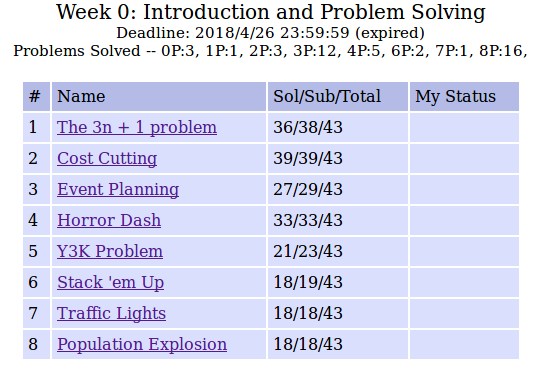
\includegraphics[width=0.8\textwidth]{img/resultW0}
    
    \bigskip

    Hope you enjoyed the warm up!
  \end{center}

\end{frame}

\begin{frame}[fragile]
  \frametitle{Comments from e-mails and questions -- 1}

  \begin{block}{Submission with Java}
    Two students had \structure{``runtime error''} with Java last week
    -- don't forget that your start class MUST be called {\bf Main}.
  \end{block}

  \vfill

\begin{verbatim}
class Main {
  public static void main(String[] args) {

    // do something...

  }
}
\end{verbatim}
\end{frame}

\begin{frame}
  \frametitle{Comments from e-mails and questions -- 2}
  \begin{block}{Input/Output}
    Two other students had problems because their program printed ``Please enter a number''.

    \bigskip

    You are very kind, but please {\bf follow the specifications} strictly!
  \end{block}
  
  \vfill

  \begin{block}{Format for MANABA submission}
    One student asked if the code for MANABA had to be the same as the code for UVA.

    \bigskip

    Yes. The code you submit on MANABA must be {\bf exactly the same}
    as the code you submitted for UVA.
  \end{block}
\end{frame}

\begin{frame}
  \frametitle{Short comments about the problems:}
  \begin{itemize}
  \item Cost Cutting, Event Planning, Horror Dash -- Easiest problems (find mean, find min, find min);
    \bigskip

  \item 3n+1 -- Still easy, but a few traps -- example of {\bf Memoization};
    \bigskip

  \item Y3K Problem -- Still easy, but skip year can be a bit troublesome.
    
  \end{itemize}
\end{frame}

%\begin{frame}
%  \frametitle{Comments about the problems}
%\end{frame}


\subsection{Outline}

\begin{frame}
  \frametitle{}

  \begin{center}
    {\large Data Structures}\\
    CP Book Chapter 2
  \end{center}
\end{frame}


\begin{frame}
  \frametitle{Motivation: Why study data structures?}

  \begin{block}{Correct Data Structure makes the problem {\bf Easier}}
    \begin{itemize}
    \item The program becomes simpler;
    \item Less Bugs;
    \item Solution becomes faster;
    \item Other good things
    \end{itemize}
  \end{block}

  \bigskip

  \begin{center}
    
\includegraphics[width=0.8\textwidth]{../img/pipeline}
  \end{center}

  \bigskip

  In this class, we will focus on {\bf implementation}. See the ``Data
  Structures'' class for the theory.  
\end{frame}

\begin{frame}
  \frametitle{Example 1: 8 Queen Problem (UVA 750)}

  \begin{columns}
    \column{0.25\textwidth}  
    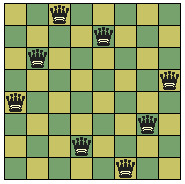
\includegraphics[width=1\textwidth]{../img/8queen}
    \column{0.75\textwidth}

    How to represent a solution?

    \vfill

    {\small
    \begin{itemize}
    \item Queen $i$ at position $x,y \rightarrow (64! / 56!)$ total solutions
      
      \bigskip
      
    \item Queen $i$ at column $c \rightarrow 8^8$ total solutions
      
      \bigskip
      
    \item Permutation of rows $ \rightarrow 8!$ total solutions
    \end{itemize}}
  \end{columns}

  \vspace{3cm}
  
  \hrulefill\\
  {\tiny\hfill Image by Lee Daniel Crocker. CC-BY-SA 3.0}
\end{frame}

\begin{frame}
  \frametitle{Example 2: The Towers of Hanoi}
  
  \begin{center}
    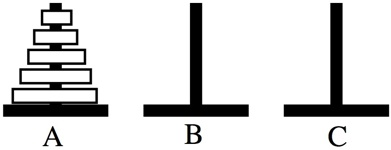
\includegraphics[width=0.5\textwidth]{img/hanoi}
  \end{center}
  \medskip

  {\small
    \begin{itemize}
    \item You have $N$ disks and $K$ poles. Each disk has unique size $s_i$.
    \item A disk $i$ can be moved from one pole to another.
    \item A move of disk $i$ to pole $k$ is only valid if $k$ has no disks smaller than $i$
    \item Find the list of moves to move all disks from pole 1 to pole $K$.
    \end{itemize}
  }
  
  \vfill

  How do you represent the data in this problem?
\end{frame}

\begin{frame}
  \frametitle{Another way to visualize the Towers of Hanoi}
  \begin{center}
    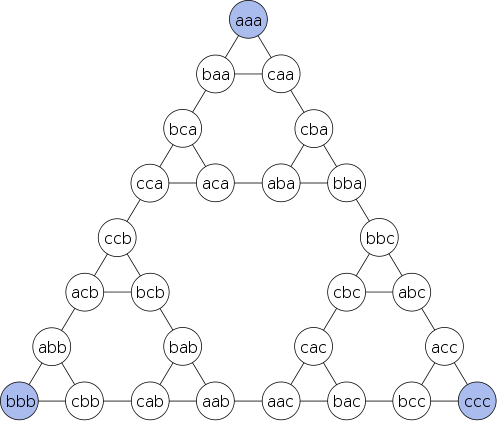
\includegraphics[width=0.7\textwidth]{img/hanoi_graph}
  \end{center}
  {\tiny \hfill Image created by nonenmac}
\end{frame}

\begin{frame}
  \frametitle{Explaining the Tower of Hanoi Data Structure}
  \begin{columns}[c]
    \column{0.7\textwidth}
    {\small
    \begin{itemize}
    \item Each node identifies one state in the problem;
    \item The string represents the position of each disk;
    \item At most {\bf Three} state transitions at any time;
    \item We can solve the problem from {\bf any start state} to {\bf
      any end state};
    \item Just find a path between the states!
    \item (just beware of state explosion)      
    \end{itemize}
    }
    \column{0.3\textwidth}    
    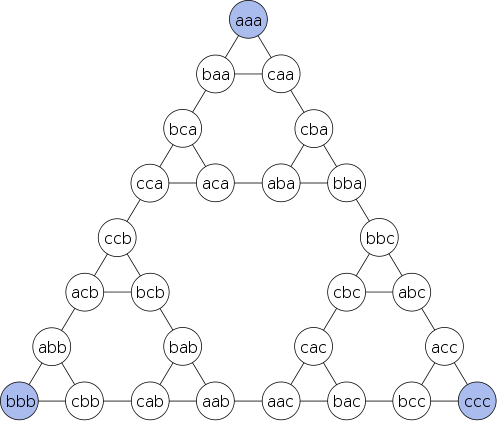
\includegraphics[width=0.9\textwidth]{img/hanoi_graph}
    \vfill
  \end{columns}
\end{frame}

\begin{frame}
  \frametitle{One Important Reminder:}

  \begin{block}{Know your libraries!}
    Array, Tree, Vector, Matrix, Graph... How do you implement them?

    \bigskip

    Most of these have standard functions in the library (STL,
    java.util), but do you remember it?

    \bigskip

    Use it many times until you don't need to google anymore.
  \end{block}

  \vfill
  
  \begin{exampleblock}{}
    Complex data structures (trees, edge matrices) are great
    candidates for your \structure{personal library}!
  \end{exampleblock}
\end{frame}

\section{Arrays and Vectors}
\subsection{Basics}

\begin{frame}
  \frametitle{The simple array!}
  Arrays are the simplest data structure, but also the most often used.

  \bigskip
  
  \begin{itemize}
  \item Preserve \emph{Programmer Efficiency}
  \item No worries about pointers;
  \item Random access;
  \item Library Functions;
  \end{itemize}
\end{frame}

\begin{frame}
  \frametitle{Make arrays, not lists}

  \begin{block}{Example: Army Buddies (12356)}
    A line of soldiers, each soldier must know who is in his {\bf
      left} and {\bf right} neighbor.

    \medskip
    
    If some soldier dies, you need to {\bf update} the left and right
    neighbors.
  \end{block}

  \medskip

  \only<1>{\structure{Linked List Approach:} Regular idea.}
  \only<2>{\structure{Array Approach:} $L[R[r]] = L[l]; R[L[l]] = R[r];$}

  \begin{center}
  \includegraphics<1>[width=0.5\textwidth]{img/army-list}
  \includegraphics<2>[width=0.8\textwidth]{img/army-array}
  \end{center}
\end{frame}

\begin{frame}[fragile]
  \frametitle{Implementing arrays}
  {\small
\begin{verbatim}
#include <vector>         // for C++ vectors

int arr[5] = {7,7,7};     // arr = {7,7,7,0,0}
vector<int> v(5, 5);      // v = {5,5,5,5,5}

int x = arr[2] + v[2];    // x = 12

arr[5] = 5;               // Runtime error
cout << v[7];             // 0 !! Be careful.

v.push_back(6);           // v = {5,5,5,5,5,6}
\end{verbatim}
  }

  \begin{block}{}
    Learn the different functions of your language of choice!
  \end{block}
  
\end{frame}

\begin{frame}[fragile]
  \frametitle{Implementation Matters: Resetting}
{\small
\begin{verbatim}
#include <vector>
#include <string.h>

vector<int> v(10000,7)

memset(v, 0, 10000*__SIZEOF_INT__);       // Method 1
fill(v.begin(), v.end(), 0);              // Method 2
for (int i = 0; i < 10000; i++) v[i] = 0; // Method 3
v.assign(v.size(), 0);                    // Method 4


Method      |  executable size  |  Time Taken (in sec) |
            |  -O0    |  -O3    |  -O0      |  -O3     |  
------------|---------|---------|-----------|----------|
1. memset   | 17 kB   | 8.6 kB  | 0.125     | 0.124    |
2. fill     | 19 kB   | 8.6 kB  | 13.4      | 0.124    |
3. manual   | 19 kB   | 8.6 kB  | 14.5      | 0.124    |
4. assign   | 24 kB   | 9.0 kB  | 1.9       | 0.591    |
\end{verbatim}
}
\end{frame}
  

\subsection{Queue and Stack}

\begin{frame}[fragile]
  \frametitle{Queue and Stacks}

  \begin{block}{}
    Queues and Stacks are useful to simplify common cases of vectors
  \end{block}

  Queue example: List of nodes to visit in pathfinding
{\small
\begin{verbatim}
#include <queue>
#include <vector>
#include <utility>

// index and neighbor list
queue <pair <int, vector <int>>> visit_list;

// ... data initialization

pair <int, vector <int>> cur = visit_list.front();

for (int i = 0; i < neighbor[cur.first]; i++)
   visit_list.push(cur.second[i]);
\end{verbatim}
}
  
\end{frame}

\begin{frame}[fragile]
  \frametitle{Queue and Stacks}

  \begin{block}{}
    Queues and Stacks are useful to simplify common cases of vectors
  \end{block}

  Stack Example: Testing if a set of parenthesis is balanced.
{\small
\begin{verbatim}
#include <stack>
stack<char> s;
char c;

while(cin >> c) {
  if (c == '(') s.push(c);
  else { 
    if (s.size() == 0) { s.push('*'); break; }
    s.pop();
  }
}
cout << (s.size() == 0 ? "balanced" : "unbalanced");

\end{verbatim}}
\end{frame}



\subsection{Sorting}
% Sorting
\begin{frame}
  \frametitle{Sorting}

  Sorting is an extremely important operation. Many algorithms begin
  or end with sorting the data.

  \bigskip
  
  {\small
    \begin{itemize}
    \item Finding the n-th highest value;
    \item Finding duplicate values;
    \item Pre-processing data for binary search;
    \item etc...
    \end{itemize}
  }
  
  
  \begin{block}{}
    You should know how to sort in your chosen language with your eyes closed!
  \end{block}
  
  % A very important operation on arrays is sorting
  % You should get used to doing it with your eyes closed!
\end{frame}
  
\begin{frame}[fragile]
  \frametitle{Sorting Example -- Vito's Family (UVA 10041)}
  
  \begin{exampleblock}{Problem description}
    A gangster is looking for a new house. The distance from the new
    house to {\bf each and all} family members should be minimal.
  \end{exampleblock}

  \medskip

  This program can be summarized as ``find the median of the addresses
  and calculate the distance to all the houses.''

  \medskip

  \begin{block}{}
    {\small
\begin{verbatim}
#include <algorithm>

int addr[m] // positions (0-5000) of each house.
// read positions from input.

sort(addr,addr+m); 
// if vector, sort(addr.begin(), addr.end())
med = add[(m/2)];
\end{verbatim}}
  \end{block}
\end{frame}

\begin{frame}[fragile]
  \frametitle{Sorting with specific sorting function}
  \begin{block}{}
    Remember, in the function, the main comparison should come first.
  \end{block}

  {\small
\begin{verbatim}
#include <algorithm>
#include <vector>
#include <string>
struct team{ string n; int p; int g; 
             team(string _n, int _p, int _g) : 
                n(_n), p(_p), g(_g){} };

bool cmp(team a, team b) {
  if (a.p != b.p) return a.p < b.p;
  if (a.g != b.g) return a.g > b.g;
  return 1; }

vector<team> v;
sort(v.begin(), v.end(), cmp); // sort using cmp
reverse(v.begin(), v.end()); // and reverse
\end{verbatim}}
\end{frame}

\begin{frame}
  \frametitle{To sort or not to sort?}

  Let's say we want to find an specific value $k$

  \bigskip
  
  \begin{block}{Checking each value in the array with $n$ elements}
    \begin{itemize}
    \item Cost for searching once: $O(n)$
    \item Cost for searching $m$ times {\bf in the same array}: $O(m*n)$
    \end{itemize}
  \end{block}

  \begin{alertblock}{Sort and binary search}
    \begin{itemize}
    \item Cost for searching once: $O(n\text{log}n + \text{log}n)$
    \item Cost for searching $m$ times in the same array: $O(n\text{log}n + m\text{log}n)$
    \end{itemize}
  \end{alertblock}
  
  \bigskip

  The best one depends on the problem!
\end{frame}

\begin{frame}[fragile]
  \frametitle{Binary Search}
  
  {\small You can use algorithm::lower\_bound and algorithm::upper\_bound
   
  \begin{block}{}
\begin{verbatim} 
#include <iostream>     
#include <algorithm>    
#include <vector>       
int main () {
  int myints[] = {10,20,30,30,20,10,10,20};
  vector<int> v(myints,myints+8);           
  sort (v.begin(), v.end());                

  vector<int>::iterator low,up;
  low= lower_bound (v.begin(), v.end(), 20); 
  up = upper_bound (v.begin(), v.end(), 20); 

  cout <<"lower at "<<(low-v.begin())<< '\n';
  cout <<"upper at "<<(up -v.begin())<< '\n';

  return 0; // up and low are memory indexes. }
\end{verbatim}
    \end{block}
}
\end{frame}


\section{Other Data Structures}
\subsection{Maps}

\begin{frame}
  \frametitle{Maps and Sets}

  Maps and sets are useful if you have a group of unique items. It
  is easy to test for the {\bf Presence of Abscense} of a particular
  item.

  \vfill

  Also, if the number of elements is too large (example, problem CD),
  maps are usually really fast.
  
\end{frame}

\begin{frame}[fragile]
  \frametitle{Map implementation (1)}
  {\small
\begin{verbatim}
#include <map>
#include <set>

set<int> used_values;      used_values.clear();
map<string, int> mapper;   mapper.clear();

mapper["john"] = 78;   used_values.insert(78);
mapper["billy"] = 69;  used_values.insert(69);
mapper["andy"] = 80;   used_values.insert(80);
mapper["steven"] = 77; used_values.insert(77);
mapper["felix"] = 82;  used_values.insert(82);

for (map<string, int>::iterator it = mapper.begin(); 
     it != mapper.end(); it++) {
    cout << " " << ((string)it->first).c_str();
    cout << " " << it->second; 
} 
\end{verbatim}}
\end{frame}

\begin{frame}[fragile]
  \frametitle{Map implementation (2)}
  {\small
\begin{verbatim}
// interesting usage of lower_bound and upper_bound
// display data between ["f".."m") ('felix', 'john')
for (map<string, int>::iterator it = 
     mapper.lower_bound("f"); 
     it != mapper.upper_bound("m"); it++)
  printf("%s %d\n", 
         ((string)it->first).c_str(),
         it->second);

// O(log n) search of a value:
set<int>::iterator f = used_values.find(79);
if (f == used_values.end())
  cout << "not found!\n";
else
  cout << *f;
\end{verbatim}}
\end{frame}

\subsection{Union-Find}
\begin{frame}
  \frametitle{Union-Find Disjoint Set}

  \begin{block}{}
    Sometimes we need to create our own data sets.
  \end{block}

  \bigskip

  \begin{itemize}
  \item The UFDS represent a {\bf set of items} that can be in one of many {\bf groups}

    \bigskip
    
  \item For example, we can have a set of {\bf people} who can be in one of many {\bf families}

    \bigskip

  \item This can be useful to finding {\bf unconnected components} in graphs

    \bigskip

  \item A good implementation of UFDS can test if a item belongs to a group in close to O(1);    
  \end{itemize}
\end{frame}

\begin{frame}[fragile]
  \frametitle{UFDS Implementation (1/3) }

  {\small
\begin{verbatim}
typedef vector<int> vi; // use shorthand for vectors

class UnionFind { 
private: 
  vi p, rank, setSize;  // vi -- vector <int>
  int numSets;
public:
  UnionFind(int N) {
    setSize.assign(N, 1); // each element in a set 
    numSets = N; 
    rank.assign(N, 0);    // everyone is root
    p.assign(N, 0); 
    for (int i = 0; i < N; i++) p[i] = i; }

  int findSet(int i) { 
    return (p[i] == i) ? i : (p[i] = findSet(p[i])); }
\end{verbatim}
  }
\end{frame}
\begin{frame}[fragile]
  \frametitle{UFDS Implementation (2/3)}

  {\small
\begin{verbatim}             
  // continue UnionFind class

  bool isSameSet(int i, int j) 
     { return findSet(i) == findSet(j); }
  void unionSet(int i, int j) { 
    if (!isSameSet(i, j)) { numSets--; 
    int x = findSet(i), y = findSet(j);
    // rank is used to keep the tree short
    if (rank[x] > rank[y]) 
      { p[y] = x; setSize[x] += setSize[y]; }
    else                   
      { p[x] = y; setSize[y] += setSize[x];
        if (rank[x] == rank[y]) rank[y]++; } } }
  int numDisjointSets() { return numSets; }
  int sizeOfSet(int i) { return setSize[findSet(i)]; }
};
\end{verbatim}}
\end{frame}

\begin{frame}[fragile]
  \frametitle{UFDS Implementation (3/3)}

  {\small
\begin{verbatim}
int main() {
  UnionFind UF(5); // create 5 disjoint sets
  printf("%d\n", UF.numDisjointSets()); // 5
  UF.unionSet(0, 1);
  printf("%d\n", UF.numDisjointSets()); // 4
  UF.unionSet(2, 3);
  printf("%d\n", UF.numDisjointSets()); // 3
  UF.unionSet(4, 3);
  printf("%d\n", UF.numDisjointSets()); // 2
  printf("isSameSet(0, 3) = %d\n", UF.isSameSet(0, 3)); 
    // will return 0 (false)
  printf("isSameSet(4, 3) = %d\n", UF.isSameSet(4, 3)); 
    // will return 1 (true)
  UF.unionSet(0, 3);
  printf("%d\n", UF.numDisjointSets()); // 1
}
\end{verbatim}
}
  
\end{frame}


\subsection{Bitmasks}

\begin{frame}[fragile]
  \frametitle{Using Bitmasks}
  {\smaller
  A \structure{bitmask} is a lightweight version of a
  \structure{bitset}. You can use an unsigned integer or an unsigned
  long directly as a proxy for a bitset.

  \begin{block}{}
\begin{verbatim}
#include <iostream>

using namespace std;

int main() {
    unsigned long bb = 3432;
    unsigned long kk = 14;
    cout << (bb & kk) << endl;
    cout << (bb << 3) << endl;
}
\end{verbatim}
  \end{block}

  In a programming contest, they are very useful for quickly
  manipulating sets (specially if you need to modify a large number of
  members at the same time).
  }
\end{frame}

\begin{frame}[fragile]
  \frametitle{When to use bitmasks} 
  
  {\smaller In programming challenges, bitmasks are useful for quickly
    manipulating sets of items. Specially if you need to modify
    multiple sets at the same time.  

    \begin{block}{}
      $S = 34 = 100010$\\
      \medskip
      Can be seen as a set with elements 1 and 5 present.\\ 
      The index increase with the digit significance.
    \end{block}
    
    \bigskip

    In regular programming, bitmasks are often used to quickly
    set/check flags or options.
    
    \begin{block}{Bitmasks in regular programming}
      \begin{itemize}
      \item Parameter setting/testing
\begin{verbatim}
Gdx.gl.glClear( GL20.GL_COLOR_BUFFER_BIT | 
                GL20.GL_DEPTH_BUFFER_BIT );
\end{verbatim}
      \item Collision/Filtering in computer graphics
\begin{verbatim}
if( isFilled(sprite1Pixel) && isFilled(sprite2Pixel))
    return true;
\end{verbatim}
      \end{itemize}
    \end{block}
  }
\end{frame}

\begin{frame}[fragile]
  \frametitle{Binary Operatons on Bitmasks (2)}
{\smaller

  \begin{itemize}
  \item Multiply/Divide an integer by two :: shift bits left, right
\begin{verbatim}
S          = 34       =  100010
S = S << 1 = S*2 = 68 = 1000100
S = S >> 2 = S/4 = 17 =   10001
S = S >> 1 = S/2 =  8 =    1000
\end{verbatim}
\item To check if the ith item is on the set, use bitwise AND
  operation, (T = S \& (1 << j)) and test if the result is not zero.
\begin{verbatim}
S          = 34       =  100010
j = 3, 1 << j         =  001000
i = 1, 1 << 1         =  000010
                         ------
Tj= S & ( 1 << j)     =  000000  = 0 # 3 is not set
Ti= S & ( 1 << i)     =  000010 != 0 # 1 is set
\end{verbatim}

  \end{itemize}

}
\end{frame}

\begin{frame}[fragile]
  \frametitle{Binary Operations on Bitmasks (2)}
  {\smaller
  \begin{itemize}
  \item To set/turn on the jth item, use bitwise OR operation S |= (1 << j)
\begin{verbatim}
S          = 34       =  100010
j = 3, 1 << j         =  001000
                         ------ OR (S |= 1 << j)
S          = 42       =  101010
\end{verbatim}
\item To set/turn off the jth item, use bitwise AND operation S \&= ~(1 << j)
\begin{verbatim}
S          = 50       =  110010
j = (1<<5)|(1<<3)     =  101000 # unset items 5,3 
~j                    =  010111
                         ------
S &= ~(j)             =  010010 # 18
\end{verbatim}
  \end{itemize}

  }
\end{frame}

\begin{frame}[fragile]
  \frametitle{Have some code with the previous examples!}
  {\smaller
\begin{verbatim}
#include <iostream>
using namespace std;

int main() {
    unsigned int S = 34;    
    cout << (S<<1) << endl;
    cout << ((S<<1)>>2) << endl;
    cout << (((S<<1)>>2)>>1) << endl << endl;    
    cout << (S & (1 << 3)) << endl;
    cout << (S & (1 << 1)) << endl << endl;    
    cout << (S | (1 << 3)) << endl;    
    S = 50;
    cout << (S & ~((1 << 5)|(1<<3))) << endl;
}
\end{verbatim}

  }
\end{frame}


\begin{frame}[fragile]
  \frametitle{Bitsets}
  {\smaller

  Bitsets can also be used in place of integer bitmasks:

  \begin{block}{}
\begin{verbatim}
#include <bitset>
#include <iostream>

using namespace std;

int main() {
    bitset<12> b(3432);
    cout << "3432 in binary is " << b << endl;
    
    bitset<12> k(14);
    cout << (b & k) << endl;
    cout << (b<<3) << endl;
}
\end{verbatim}
  \end{block}
  }
\end{frame}

\begin{frame}
  \frametitle{Bitsets and Bitmasks}

  {\smaller
  Most bitmask operations are also supported by bitsets. (But you can't mix them!)

  \begin{itemize}
  \item All binary operations are supported;
  \item Bitsets are of fixed size, but not limited to 32 and 64 bits.
  \item Bitset standard output is a bit string, not a decimal (but
    outputing a decimal is possible);
  \item But maybe bitmasks are more efficient?
  \end{itemize}
  
  More information about bitmasks 

  \url{http://www.drdobbs.com/the-standard-librarian-bitsets-and-bit-v/184401382}
  }
\end{frame}

\subsection{Other Examples}
\begin{frame}
  \frametitle{And many more examples}

  These are just a few examples of data structures that are common in
  programming challenges. There are many more that you should study
  and add to your library. For example:

  \bigskip

  \begin{itemize}
  \item Binary Tree (2.3)
  \item Segment Tree (2.4.3)
  \item Hashing (2.3)
  \item etc...
  \end{itemize}
\end{frame}

\section{Extra}
\subsection{Problem Hints}

\begin{frame}
  \frametitle{}

  \begin{center}
    Hints
  \end{center}
  
\end{frame}

\begin{frame}
  \frametitle{Jolly Jumpers}
  Test a ``jolly'' sequence.
  \begin{itemize}
  \item Very easy problem, convert the input correctly?
  \item Do you need to store the input values?
  \item What information do you need to memorize?
  \end{itemize}
\end{frame}

\begin{frame}
  \frametitle{Newspaper}

  This is an example of a {\bf DAT} -- Direct Address Table -- a kind
  of hashing.

  \bigskip

  Be careful that any symbol can appear in the text -- negative values
  from signed chars are a common source of bugs.
  
\end{frame}

\begin{frame}
  \frametitle{Army Buddies}

  We need to keep track of changes in the neighbors of the
  soldiers.

  \bigskip
  
  The time limit is very tight.

  \bigskip

  You cannot afford to use a O(n) method to update the army.

  \bigskip

  One idea is the two-array structure discussed earlier.
\end{frame}

\begin{frame}
  \frametitle{Grid Successors}

  In this exercise, you need to find a loop in the sequence of grids.

  \bigskip

  What is the easiest structure to store this loop?
  
\end{frame}

\begin{frame}
  \frametitle{Football (aka Soccer)}

  The problem is easy, but you need to know the library to deal with
  the complex input.
\end{frame}

\begin{frame}
  \frametitle{File Fragmentation}
  Find the original bit string.
  \begin{itemize}
  \item Understanding the problem: What are looking for here?
  \item Finding out the correct combination:
    \begin{itemize}
    \item Method1: Elimination;
    \item Method2: Counting;
    \end{itemize}
  \end{itemize}
\end{frame}

\begin{frame}
  \frametitle{CD}

  The problem is very easy: given two collections of numbers, find the
  numbers in both collections.

  \bigskip
  
  However, the input data is HUGE -- you need to use an efficient data
  structure.
\end{frame}

\begin{frame}
  \frametitle{War}

  You need to use the UFDS as a basis, but you need to add {\bf
    something extra}. This one is a challenge for you!
\end{frame}


\subsection{Fun Stuff}

\begin{frame}
  \frametitle{}

  Some Extra Stuff...
\end{frame}

\begin{frame}
  \frametitle{How many sorting Algorithms are there?}
  \begin{columns}[c]
    \column{0.5\textwidth}
    {\tiny
    \begin{itemize}
    \item bubblesort
    \item insertion sort
    \item selection sort
    \item heapsort
    \item mergesort
    \item quicksort
    \item radix sort
    \item bin sort
    \item gnome sort
    \item library sort
    \item comb sort
    \item tree transversal
    \item sorting networks
    \item cocktail shaking sort
    \item bucket sort
    \item bogo sort
    \item bitonick sort
    \item ...
    \item And many more!
    \end{itemize}}
    \column{0.5\textwidth}
    \includegraphics<2>[width=1\textwidth]{../img/fliptable}
  \end{columns}
\end{frame}

\begin{frame}
  \frametitle{What do sorting algorithms sound like?}

  sorting.mp4
  
\end{frame}

\end{document}
